
\documentclass[10pt,a4paper]{article}
%\usepackage[cm]{fullpage}
\usepackage[danish]{babel}
\usepackage[utf8]{inputenc}
%\usepackage[margin=1.1cm]{geometry}
\usepackage[top=1.5cm, bottom=1.2cm, left=1.2cm, right=1.2cm]{geometry}
%\usepackage[official]{eurosym}
%\usepackage{eso-pic}
\usepackage{tikz}
\usepackage{pgffor}
\usepackage{graphicx}%,epic,eepic}
\usepackage{amssymb}
\usepackage{textcomp}
\usepackage{amsmath}
\usepackage{amsmath, amsthm, amssymb}
\usepackage{latexsym}
%\usepackage[usenames,dvipsnames]{color}
\usepackage{float}
\usepackage{calc}
\usepackage{pdfpages}
\usepackage{epstopdf}
\usepackage{caption}
\usepackage{subcaption}
\usepackage{url}
\usepackage{fancyhdr}
\usepackage{hyperref}
\usepackage{nameref}
\usepackage{setspace}
% \usepackage{slashbox}
\usepackage{color, colortbl}
\usepackage{microtype}
\usepackage{vwcol}
\usepackage{lipsum}
\usepackage{xcolor}
\usepackage{xparse}
\usepackage{changepage}

\ExplSyntaxOn
\NewDocumentCommand{\makebullet}{ m }
 {
  \clist_map_inline:nn { #1 } { $\bullet$ \hspace{0.1cm} ##1 \hspace{0.2cm} }
 }
\ExplSyntaxOff

\definecolor{MyColor}{rgb}{0.83,0.87,0.94}
\makeatletter\newenvironment{Colorbox}{%
   \begin{lrbox}{\@tempboxa}\begin{minipage}{\columnwidth}}{\end{minipage}\end{lrbox}%
   \colorbox{MyColor}{\usebox{\@tempboxa}}
}\makeatother

\newlength{\mylen}
\newcommand{\myflexbox}[2][7em]{%
  \settowidth{\mylen}{#2}%
    \makebox[#1][l]{#2}%
}

\newcommand{\dunderline}[1]{\underline{\underline{#1}}}
\newcommand{\bea}{\begin{eqnarray}}
\newcommand{\eea}{\end{eqnarray}}
\newcommand{\bcb}{\begin{Colorbox}}
\newcommand{\ecb}{\end{Colorbox}}
\newcommand{\Repeat}[2]{% \repeat already defined
    \foreach \n in {1,...,#1}{#2}
}
\newcommand{\newprojects}[3]{\\\textbf{#1}\\#2\\ \makebullet{#3}\\}
\newcommand{\textline}[3]{\textbf{#1} #2 \hfill \textit{#3}}

%\newcommand{\proficiencysquare}[2]{\tikz \node (rect) at (0,0) [draw,minimum width=(\columnwidth - \widthof{#1})/20,minimum height=4pt,fill=#2!100] {};\hspace{2pt}}
\newcommand{\proficiencysquare}[3]{\tikz \node (rect) at (0,0) [draw=none,minimum width=(\columnwidth - #1)/20,minimum height=4pt,fill=#2!40] {};\hspace{#3}}

\newcommand{\proficiencycircle}[3]{\tikz \node at (0,0) [circle,inner sep=0pt,minimum width=(\columnwidth - #1)/20,fill=#2] {};\hspace{#3}}

\newcommand{\proficiency}[3]{#1\Repeat{#2}{\proficiencysquare{#1}{#3}}}

\newcommand{\proficientsquare}[5]{\myflexbox{#1}\Repeat{#2}{\proficiencysquare{#3}{#4}{#5}}}

\newcommand{\proficientcircle}[5]{\myflexbox{#1}\Repeat{#2}{\proficiencycircle{#3}{#4}{#5}}}

\usepackage[defaultfam,light,tabular,lining]{montserrat} %% Option 'defaultfam'
%% only if the base font of the document is to be sans serif
\usepackage[T1]{fontenc}
\renewcommand*\oldstylenums[1]{{\fontfamily{Montserrat-TOsF}\selectfont #1}} % Only if the base font of the document is to be sans serif

\definecolor{carmine}{rgb}{0.59, 0.0, 0.09}
\definecolor{coralred}{rgb}{1.0, 0.25, 0.25}
\definecolor{darkscarlet}{rgb}{0.34, 0.01, 0.1}
\definecolor{myblue}{rgb}{0.0, 0.43, 0.59}

\newcommand{\headline}[1]{\Large \textcolor{myblue}{#1}}

\newcommand{\skillcolor}{myblue}

\newcommand{\skillbar}[2]{%
    \ifthenelse{%
        \equal{#2}{0}%{%
    }{\Repeat{5}{\proficiencycircle{0.5pt}{\skillcolor}{2.0pt}}}%
    {\Repeat{#1}{%
                \proficiencycircle{0.5pt}{\skillcolor}{2.0pt}%
            }\hspace{-3pt}\Repeat{#2}{%
                \proficiencycircle{0.5pt}{lightgray}{2.0pt}%
            }%
        }%
    }

\newcommand{\accomplishment}[1]{{\hspace*{-9pt}\textcolor{myblue}{$\bullet$}}\hspace*{4pt}\linespread{1.1}\footnotesize#1}

%\usepackage{blindtext}

\linespread{1.0}

\begin{document}
\pagenumbering{gobble}
%\fontfamily{cmss}
\parindent0em
%\fontfamily{qag}
%\fontfamily{verdana}
\begin{minipage}[t]{0.5\linewidth}
\vspace{-3.85cm}
{\Huge \textcolor{myblue}{Rógvi Dávid Arge} }\\

{\Large \mbox{Data Science \& Optimization Consultant}}
\vspace{0.3cm}

Phone: +45 5042 5002

\vspace{0.1cm}
E-mail: argeinnovations@gmail.com

\vspace{0.1cm}
LinkedIn: \url{http://dk.linkedin.com/in/rogvidarge/en}

\vspace{0.1cm}
GitHub: \url{https://github.com/rogvid} \\
%Portfolio: \url{https://rogvid.github.io}
\vspace{-1.6cm}
\end{minipage}\hspace{0.1cm}
\hfill\begin{minipage}[t]{0.3\linewidth}\raggedleft
    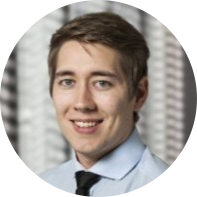
\includegraphics[width=0.7\columnwidth]{workpicture.png}
\end{minipage}

\vspace{0.9cm}
\hrule height 0.4mm
\vspace{0.5cm}
{\headline{SUMMARY}}\\
Data Science Consultant with 3+ years experience in agile project development and a passion for machine learning and optimization. Vast experience in data wrangling, exploratory data analysis, machine learning and data visualization and applying these skills to generate corporate wide improvements. Expert at involving- and making the business take ownership of projects.\\
\vspace{0.3cm}
\\
  \begin{minipage}[t]{0.66\linewidth}
    %{\Large \textcolor[HTML]{777777}{EXPERIENCE}}\\
    {\headline{EXPERIENCE}}\\
    \vspace{-8pt}\\
    \textbf{Arge Innovations} $|$ Owner \& Data Science Consultant \hfill \textit{Dec. 2018 -} \\
    Agile development and deployment of data science, and optimization products.\\
    \newprojects{Arge Innovations $|$ Data Science Consultant - DFDS A/S \\ Projects \hfill \textmd{\textit{Dec. 2018 - May. 2019}}}%
        \\%
            \accomplishment{Scoped, developed, and deployed an optimization algorightm for transport operations}\\%
            \accomplishment{Deployed dockerized Flask APIs and Frontends to DFDS Kubernetes cluster}%
        }{}
    \normalsize \textbf{ATP=} $|$ Data Scientist \hfill \textit{Feb. 2017 - Dec. 2018} \\
    \accomplishment{Developed database monitoring system essential for our day to day work. We never missed a prediction because of database downtime since then}\\
    \accomplishment{Built machine learning model for finding citizens who reported false addresses. Allowed us to find people with complex fraud patterns}\\
    \accomplishment{Developed multiple expert systems designed to capture specific types of fraudulent behaviour}\\
    %\textbf{ArgeX} $|$ Owner \& Developer \hfill \textit{Nov. 2015 -} \\
    %Develop and help design VBA macros to analyze and automize language translation\\
    \\
    \normalsize \textbf{ConWX} $|$ Programmer \& Data Analyst \hfill \textit{Apr. 2015 - Feb. 2017} \\
    \accomplishment{Discovered and validated a way to improve forecasting for our clients by 10-25\% vastly increasing client profit per month}\\
    \accomplishment{Designed and developed a monitoring system essential for forecast quality assurance and improvement}\\
    %\textbf{ArgeX} $|$ Owner \& Developer \hfill \textit{Nov. 2015 -} \\
    %Develop and help design VBA macros to analyze and automize language translation\\
    \newprojects{\normalsize{Udacity Data Analyst Nanodegree Project \\ Explore and Summarize Data \hfill \textmd{\textit{Feb. 2016}}}}{Scraped \textcolor{black}{\url{Boliga.dk}} and income statistics for people in Copenhagen. EDA showed an explosive increase in appartment prices around 500\%, as well as the effects of the economic crisis on declining size of raises.}{Python, R, MongoDB, EDA, Data Wrangling}
    \\

    {\headline{EDUCATION \& CERTIFICATION}}\\
    \vspace{-8pt}\\
    \textline{Coursera}{Deep learning}{2018}\\
    Deep Learning Specialization by Andrew Ng on the MOOC Coursera.\\
    \\
    \textline{Udacity}{Data Analyst Nanodegree}{2015 - 2017} \\
    Project based online education teaching essential knowledge and skills for data scientists.\\
    \\
    \textline{Copenhagen University}{MSc in Physics}{2012 - 2015}\\
    Focus on computational physics, machine learning and mathematical modeling.\\

  \end{minipage}\hfill\vline width 0.4mm\hfill
\begin{minipage}[t]{0.28\linewidth}
    {\headline{TECHNICAL SKILLS}}\\
    \vspace{-8pt}\\
    \hspace*{-6pt}\begin{tabular}{l l l}
        Python & \skillbar{5}{0}\\
        Machine Learning & \skillbar{5}{0}\\
        Optimization & \skillbar{5}{0}\\
        Operations Research & \skillbar{5}{0}\\
        Data Visualization & \skillbar{5}{0}\\
        Data Analysis & \skillbar{5}{0}\\
        Modeling & \skillbar{5}{0}\\
        Statistics & \skillbar{5}{0}\\
        Git & \skillbar{5}{0}\\
        SQL & \skillbar{4}{1}\\
        D3 & \skillbar{4}{1}\\
        HTML & \skillbar{4}{1}\\
        CSS & \skillbar{4}{1}\\
        JavaScript & \skillbar{3}{2}\\
        C\# & \skillbar{3}{2}\\
        Docker & \skillbar{3}{2}\\
        AWS & \skillbar{3}{2}\\
        Azure & \skillbar{3}{2}\\
        MongoDB & \skillbar{3}{2}\\
        R & \skillbar{3}{2}\\
    \end{tabular}
    \\
    \vspace{0.5cm}

    {\headline{SOFT SKILLS}}\\
    \vspace{-8pt}\\
    \hspace*{-6pt}\begin{tabular}{l l l}
        Problem Solving & \skillbar{5}{0}\\
        Critical Thinking \hspace{11pt} & \skillbar{5}{0}\\
        Communication & \skillbar{5}{0}\\
        Adaptability & \skillbar{5}{0}\\
        Project Planning & \skillbar{5}{0}\\
        Decision Making & \skillbar{5}{0}\\
        Scrum & \skillbar{4}{1}\\
    \end{tabular}
    \vspace{0.5cm}

    {\headline{LANGUAGES}}\\
    \vspace{-6pt}\\
    \textbf{Native speaker}\\
    \hspace*{-6pt}\begin{tabular}{l l l}
        Faroese & \hspace{44pt} & \skillbar{5}{0}\\
        Danish & \hspace{44pt} & \skillbar{5}{0}\\
    \end{tabular}\\
    \vspace{-2pt}

    \textbf{Professional proficiency}\\
    \hspace*{-6pt}\begin{tabular}{l l l}
        English & \hspace{44pt} & \skillbar{4}{1}\\
    \end{tabular}\\
    \vspace{-2pt}

    \textbf{Elementary proficiency}\\
    \hspace*{-6pt}\begin{tabular}{l l l}
        Norwegian & \hspace{30pt} & \skillbar{3}{2}\\
        Swedish & \hspace{30pt} & \skillbar{3}{2}\\
        French & \hspace{30pt} & \skillbar{2}{3}\\
    \end{tabular}\\
\end{minipage}
\end{document}
